\documentclass[a4paper]{article}

\usepackage[utf8]{inputenc}
\usepackage[portuges]{babel}
\usepackage{a4wide}
\usepackage{multicol}
\usepackage{spverbatim}
\usepackage{graphicx}
\usepackage{amssymb}
\usepackage{titling}



\title{Projeto de POO - UMER\\Grupo 52}
\author{Vítor Castro (A77870), Marcos Pereira (A79116), Sérgio Jorge (A77730)\\{\tiny(da esquerda para a direita)}}
\renewcommand\maketitlehooka{\pagestyle{empty}\centering\sffamily}
\renewcommand\maketitlehookc{\vskip1cm

\includegraphics[width=6cm]{grupo}
 }
\date{}

\begin{document}

\maketitle

\begin{abstract}
Neste relatório faremos uma análise do projeto de Programação Orientada aos Objetos, no qual o objetivo era desenvolver um programa, em Java, que fizesse a gestão da \textit{UMER},  uma empresa de transporte de passageiros. Assim, este documento apresenta detalhadamente a abordagem tomada ao problema proposto pela equipa docente da UC.
\end{abstract}

\tableofcontents

\section{Introdução}
\label{sec:intro}

Este projeto foi realizado com o objetivo de desenvolver um programa responsável por toda a gestão de uma empresa de taxis. Foram, então, propostas pelos professores algumas funcionalidades com contexto real enquadradas no tema, às quais o programa deve responder com sucesso. A implementação destas permitiram consolidar e adquirir conhecimentos ao nível da sintaxe de programação em Java e também incentivaram à exploração de estruturas de dados e de APIs características desta linguagem.
Assim, de modo a facilitar a compreensão do projeto, o relatório está dividido da seguinte forma:

\begin{description}
    \item[Secção 2 :] Problema;
    \item[Secção 3 :] Solução;
    \item[Secção 4 :] Conclusão.
\end{description}

\section{Problema}
\label{sec:problema}
Neste projeto de POO pede-se para desenvolver um programa capaz de auxiliar na gestão de uma empresa de transporte de pessoas. Assim, este deve ser capaz de:


\begin{itemize}
\item Registar um utilizador (cliente ou motorista);
\item Implementar login no sistema;
\item Criar viaturas;
\item Associar motoristas a viaturas;
\item Um cliente pode solicitar uma viagem escolhendo uma viatura específica ou a mais próxima de si;
\item Classificar o motorista, após a viagem;
\item Registar um utilizador (cliente ou motorista);
\item Possibilidade do cliente conseguir ver as viagens que já fez;
\item Possibilidade do motorista conseguir ver as viagens que já fez;
\item Indicar o total faturado pela viatura ou pela empresa;
\item Listar os 10 clientes que mais gastam;
\item Listar os 5 motoristas que apresentam mais desvios entre valores previstos para a viagem e o valor final faturado;
\item Gravar o estado do programa em ficheiro.

\end{itemize}

\section{Solução}
A nossa solução foi implementada com base em diferentes classes dos quais destacamos:

\begin{itemize}
    \item User;
         \begin{itemize}
         \item{Driver;}
         \item{Client;}
         \end{itemize}
    \item Vehicle;
    \item Trip;
    \item IO.
\end{itemize}
\label{sec:solucao}

\begin{figure}[htbp]
    \centering
    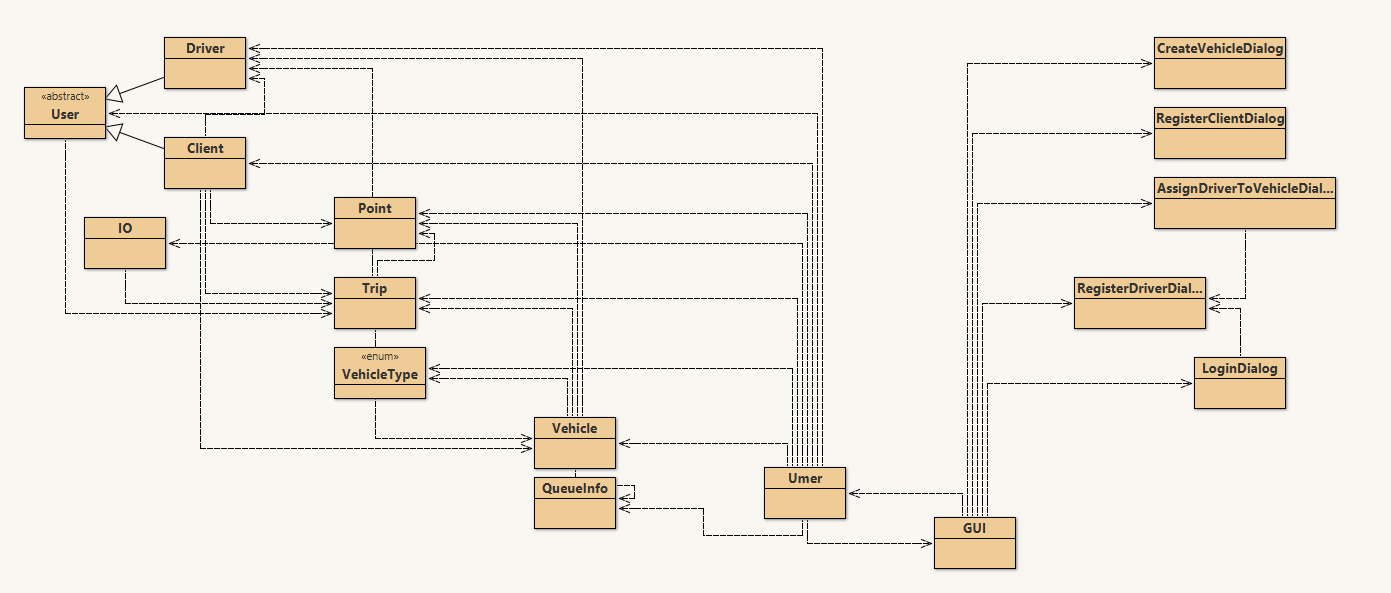
\includegraphics[width = 420pt, height = 240pt]{bluej}
\end{figure}

\pagebreak

\subsection{User}
Esta é uma superclasse que define variáveis como: email, nome, password, morada e data de nascimento do utilizador. A razão para a implementação de uma hierarquia é porque todos os campos referidos são comuns a motoristas e a clientes pelo que não há a necessidade de repetir código em diferentes classes. Está definida como abstrata porque não haverá necessidade de instanciar Users.

\begin{description}
    \item[Driver] A classe referente aos motoristas inclui as variáveis definidas na superclasse mas também o grau de cumprimento de horário, a classificação do motorista, o total de quilómetros feitos por este na empresa e um booleano que informa sobre a disponibilidade do motorista.

    \item[Client] Na classe de clientes são também incluídas as variáveis definidas em User. Além disso, define-se o ponto/localização do cliente e o dinheiro total gasto por este. Nesta classe,

\end{description}

\subsection{Vehicle}
Em Vehicle, classe relativa aos objetos táxis da empresa, são definidas variáveis como: finanças do veículo, posição, ID, tipo de veículo, motorista atual e dois booleanos relativos a fila de espera e ocupação.

\subsection{Trip}
Na classe Trip estão as variáveis relativas às viagens e, a cada viagem, deve estar associado um veículo, um motorista, dois pontos (origem e destino), duração estimada, duração real, custo da viagem , hora de partida e chegada.

\subsection{IO}
Esta é a classe responsável pelas operações de Input/Output do programa. Assim, através dela, é-nos possível guardar o estado da aplicação em determinado momento e é também possível recuperar esse estado posteriormente. O estado é guardado em ficheiros presentes na diretoria do programa.

\subsection{Implementação - UMER}

Na implementação deste programa, optamos por criar uma interface gráfica do utilizador (GUI) de modo a facilitar a interação da aplicação com as funcionalidades exigidas. Usamos três \textit{hashmaps} para guardar a informação relativa a motoristas, clientes e veículos. A escolha recaiu no uso deste tipo de estrutura de dados por nos possibilitar ganhos de performance relativamente a listas.
Por sua vez, as listas são usadas, no nosso programa, para guardar a informação relativa a viagens já completadas e viagens a decorrer.

Primeiramente, esta classe é responsável por métodos relativos a \textit{login} e \textit{logout}, instancia ou cria objetos das classes motoristas, clientes e veículos e adiciona-os às estruturas de dados respetivas e trata de associar um condutor a um veículo.
É, então, que se torna possível a criação ou o começo de uma viagem.

No que diz respeito à criação de viagens, é verificado se há algum veículo disponível ou se o que foi pedido pelo cliente está disponível. Em caso afirmativo, a viagem é adicionada às listas de viagens, as posições dos objetos são atualizadas, as finanças e o custo são adicionadas ao veículo e ao cliente e o cliente avalia o condutor. Em caso negativo, se existir algum veículo com fila de espera, o cliente é adicionado à sua fila de espera.
É importante referir que a nossa aplicação faz uso de um relógio que nos permite marcar a hora de início e de fim da viagem. Assim, é-nos possível saber quando a viagem acaba pelo que, nesse momento, podemos tirar a viagem da lista de viagens a decorrer. Está também implementado o método \textit{fastforward} que adianta o relógio.

Para cliente e motorista terem acesso às viagens que já fizeram percorre-se a lista do historial de viagens e vê-se em que viagens é que estes participaram e é apenas feito um ToString dessa informação.

Em relação aos tops, decidimos converter as \textit{hashmaps} de clientes e de motoristas para \textit{arraylists} que, posteriormente, são ordenados. A seguir, passamos os N primeiros elementos dos \textit{arraylists} (já ordenados) para \textit{linkedhashmaps} aos quais damos toString.

O estado da aplicação é guardado a partir de um botão na GUI que chama os métodos responsáveis por esse efeito, presentes na classe IO. Relativamente a carregar o estado, é feita a chamada aos métodos, automaticamente, quando a GUI é aberta.
\subsection{Resultado Final}
\begin{figure}[htbp]
    \centering
    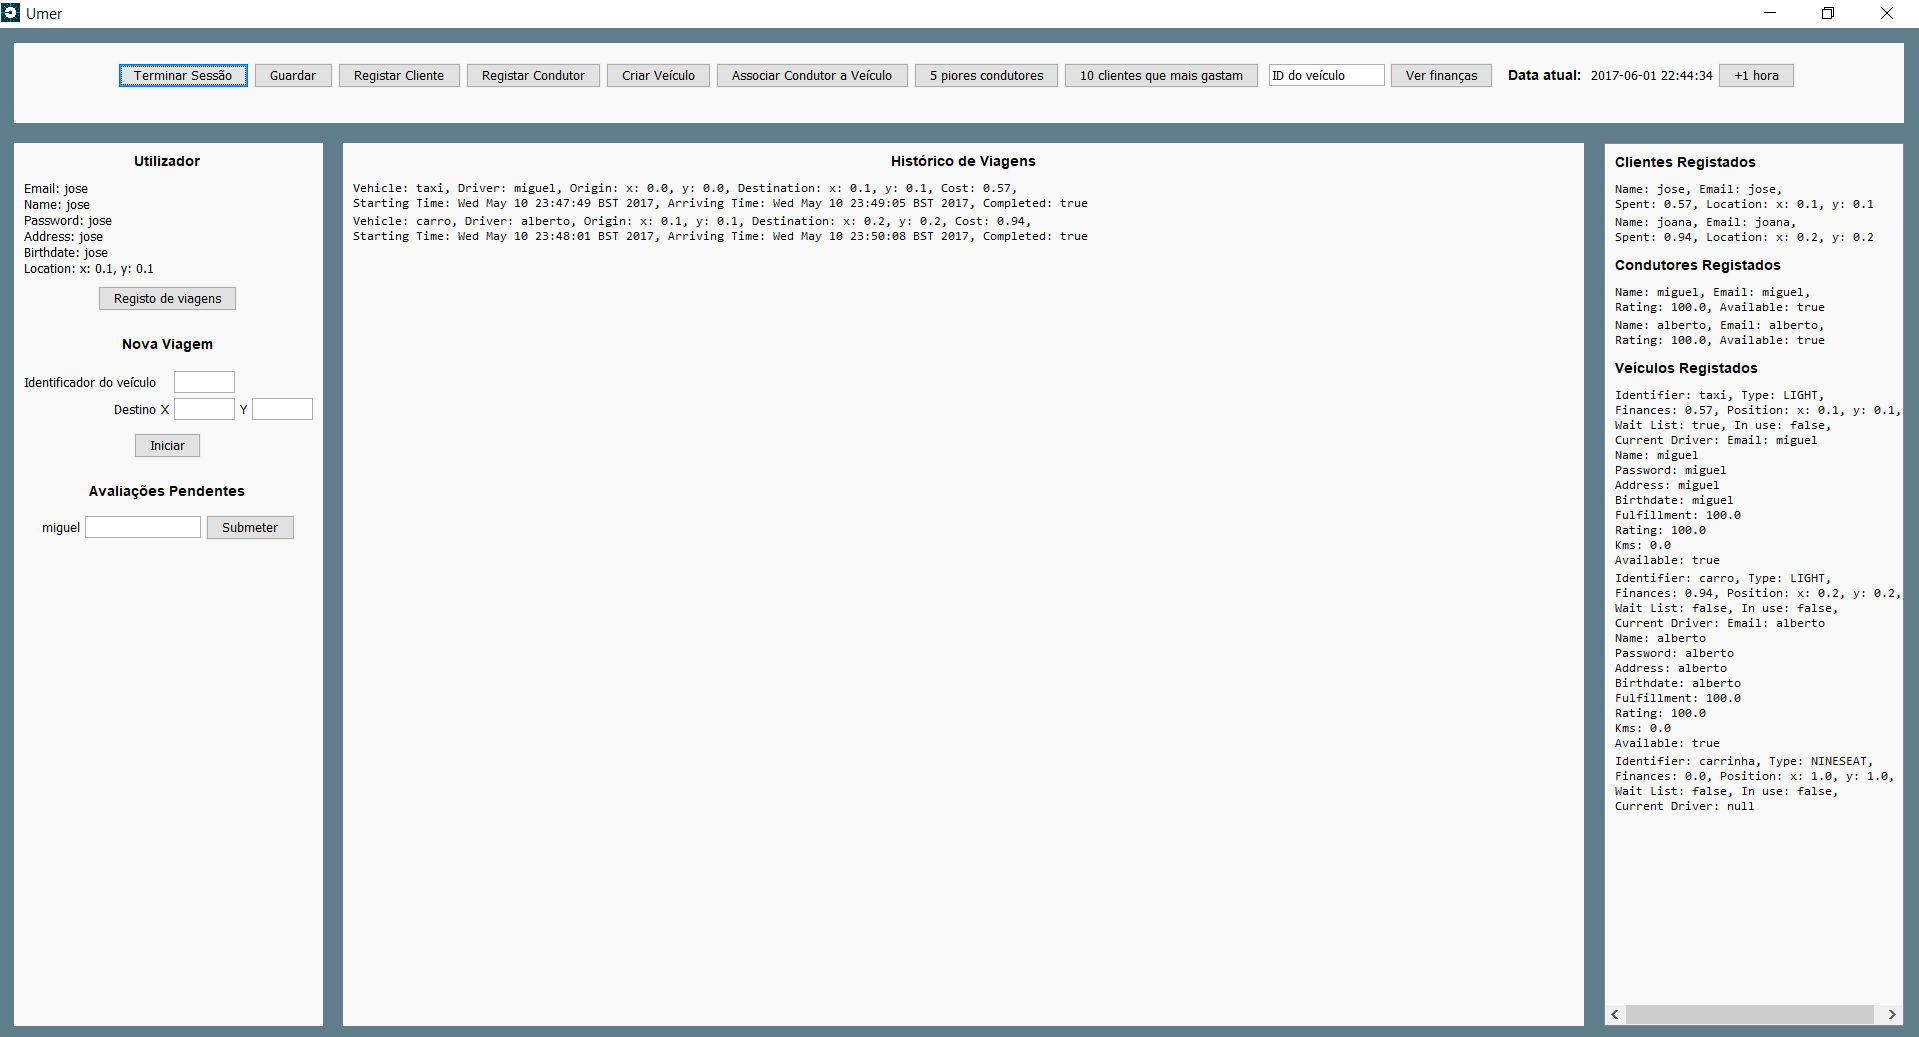
\includegraphics[width = 420pt, height = 240pt]{gui}
\end{figure}

\section{Manual de Utilização}
De seguida, se destacam os elementos que permitem proceder à utilização completa do programa, sendo que cada passo será acompanhado da devida ilustração. Todo as funcionalidades são apresentadas na mesma janela, sendo por isso fácil ter uma perspetiva completa do que acontece a cada momento.

\begin{itemize}
    \item Criar entidades;
        \begin{itemize}
        \item{Cliente;}
        \item{Condutor;}
        \item{Veículo;}
        \end{itemize}
    \item Cliente;
        \begin{itemize}
        \item{Iniciar sessão;}
        \item{Obter registo de viagens;}
        \item{Iniciar viagem;}
            \begin{itemize}
            \item{Para o veículo mais próximo;}
            \item{Para o veículo específico.}
            \end{itemize}
        \item{Avaliar motorista;}
        \item{Terminar sessão.}
        \end{itemize}
    \item Condutor;
        \begin{itemize}
        \item{Iniciar sessão;}
        \item{Obter registo de viagens;}
        \item{Alterar disponibilidade;}
        \item{Terminar sessão.}
        \end{itemize}
    \item Veículo;
        \begin{itemize}
        \item{Ver finanças.}
        \end{itemize}
    \item Outras funcionalidades.
        \begin{itemize}
        \item{Guardar o estado do programa;}
        \item{Associar condutor a veículo;}
        \item{5 piores condutores;}
        \item{10 clientes que mais gastam;}
        \item{Avançar no tempo.}
        \end{itemize}
\end{itemize}

\label{sec:manual}

\subsection{Criar entidades}
Foram disponibilizados botões específicos para cada entidade, podendo esta ser um Cliente, um Condutor ou um Veículo. Procedeu-se desta forma pois é mais intuitivo para um possível futuro utilizador. Todos as entidades registadas serão apresentadas no lado direito da janela do programa, como é visível na seguinte figura.
\begin{center}
  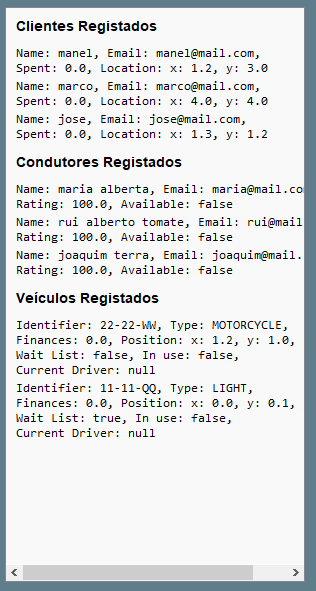
\includegraphics[scale=0.70]{janela_registados}\\
  \caption{figure}{Entidades registadas}
  \label{fig:picture}
\end{center}

\subsubsection{Cliente}
Para proceder à criação de um cliente, bastará clicar no botão "Registar Cliente", facilmente identificável no topo da interface. Depois disso, o utilizador terá de preencher os campos "Email", "Nome", "Password", "Endereço" (morada), "Nascimento" (data em qualquer formato) e "Posição" (X e Y). De seguida, clicará em "OK" e ficará registado no sistema.
\begin{center}
  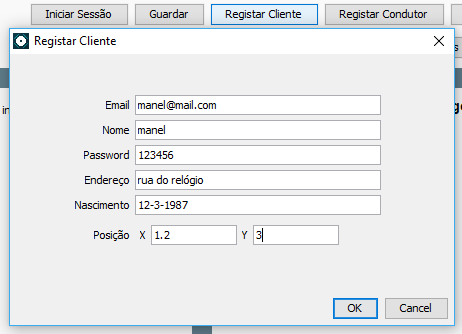
\includegraphics[scale=0.75]{criar_cliente}\\
  \caption{figure}{Criação de um Cliente}
  \label{fig:picture}
\end{center}

\subsubsection{Condutor}
Junto do botão para criação de um Cliente existe também o botão "Registar Condutor", através do qual será possível criar um novo Condutor. Obviamente, a posição do motorista não tem interesse, pelo que não é pedida.
\begin{center}
  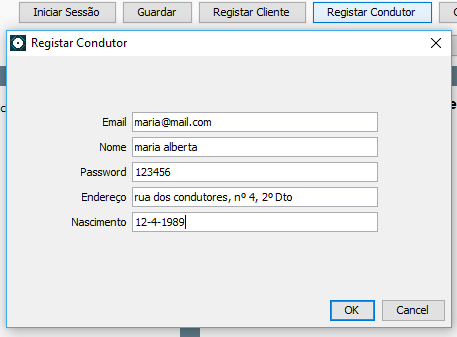
\includegraphics[scale=0.75]{criar_condutor}\\
  \caption{figure}{Criação de um Condutor}
  \label{fig:picture}
\end{center}

\subsubsection{Veículo}
Como nos anteriores, existe também um botão para a criação de um veículo - "Criar veículo". Será pedido o "Identificador" (do Veículo), o "Tipo" do mesmo (LIGHT para carros 5 lugares, NINESEAT para carros 9 lugares e MOTORCYCLE para motas), a "Posição" em que se encontra e o utilizador deverá selecionar o campo "Lista de Espera" caso pretenda que aquele veículo tenha essa característica.
\begin{center}
  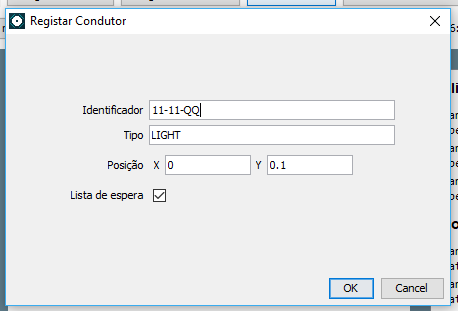
\includegraphics[scale=0.75]{criar_veiculo}\\
  \caption{figure}{Criação de um Veículo}
  \label{fig:picture}
\end{center}

\subsection{Cliente}
\subsubsection{Iniciar sessão}
\subsubsection{Obter registo de viagens}
\subsubsection{Iniciar viagem}
\paragraph{Para o veículo mais próximo}
\paragraph{Para o veículo específico}
\subsubsection{Avaliar motorista}
\subsubsection{Terminar sessão}

\subsection{Condutor}
\subsubsection{Iniciar sessão}
\subsubsection{Obter registo de viagens}
\subsubsection{Alterar disponibilidade}
\subsubsection{Terminar sessão}

\subsection{Veículo}
\subsubsection{Ver finanças}

\subsection{Outras funcionalidades}
\subsubsection{Guardar o estado do programa}
\subsubsection{Associar condutor a veículo}
\subsubsection{5 piores condutores}
\subsubsection{10 clientes que mais gastam}
\subsubsection{Avançar no tempo}


\section{Conclusões}
\label{sec:conclusao}
Este projeto serviu para aprofundarmos o conhecimento da linguagem JAVA, assim como as APIs que lhe estão associadas. Achamos que a realização de um trabalho deste tipo permite uma consolidação proveitosa da linguagem, não só em termos teóricos como também em termos práticos. Permite também melhorar as habilidades na resolução de problemas. No entanto, apesar de nos termos proposto a fazer todos os pontos do trabalho, acabamos por não ter tempo para implementar as empresas de taxis e o random dos condutores. Não temos dúvidas de que o conseguimos fazer, mas tivemos de dedicar tempo precioso a outras UCs. Fomos além do pedido e fizemos uma GUI, o que nos poderá ter custado tempo útil para fazermos os pontos pedidos que faltaram, mas acreditamos que ficamos a conhecer melhor outra parte da programação que até ao momento desconhecíamos e, assim sendo, cremos ter sido vantajoso este esforço que sabemos não contar para avaliação.

\end{document}